\documentclass[a4paper, oneside, 10pt]{article}
\usepackage{float}
\usepackage{amsfonts} % if you want blackboard bold symbols e.g. for real numbers
\usepackage{graphicx} % if you want to include jpeg or pdf pictures
\usepackage{listings} % entering code.
\graphicspath{ {images/} }

\title{{\bf 15-418 Final Project Report \\
 \large Solving Out of Core Ray Tracing Problem by a Distributed Path Tracing System}} % change this

\author{Xiao Li (xiaol2) and Yihua Eric Fang (yihuaf)}

\date{\today} % change this

\begin{document}

%%%%%%%%%% PRELIMINARY MATERIAL %%%%%%%%%%
\maketitle
\thispagestyle{empty}
\newpage
\begin{center}
\vspace*{\fill}
\section*{Abstract}
Parallel Breadth-First Search, from the past to present.\\
\vspace*{\fill}
\newpage
\end{center}

\tableofcontents
\newpage

%%%%%%%%%% MAIN TEXT STARTS HERE %%%%%%%%%%
\section{Introduction}
\section{Background}
\paragraph{} In general, the renderers used in animation, film or FX industries could be categorized as on-core and out-of-core renderers.  In the context of ray tracer, on core ray tracer ensures the whole scene to render fits in the DRAM of a machine. This allows the ray tracer to generate random numbers of rays when intersection happens, and trace them without worrying about scheduling the loading and unloading scenes. 

\paragraph{} Out-of-core renderers, on the other hand, assumes the scenes are too big to fit in the DRAM of a single machine. One of the major benefits of out-of-core renderers is they have no hard upper limits on geometries to render. However, usually the out-of-core renderers need to take extra efforts for scheduling the ray tracing system, manage the geometries workload balancing across machines, perform extra work reduction, optimization of memory coherence and hide all kinds of communication latency. 

\paragraph{} We designed a system to perform out-of-core rendering, based on Azurender, a ray tracing based renderer. We designed and implemented two algorithms. Different from the design of Hyperion or Pantaray, which are more focused on smarter sorting, loading and unloading of rays, ray packets or BVHs to hide the latency caused by hard disk accessing, our design load the scenes into DRAMs in a distributed system and focus on the scheduling and optimization for inter-machine communications. 

\section{System Design}
\subsection{System Overview}
\subsubsection{Ray Tracing System}
\paragraph{} Our system involves a basic ray tracing logic, as shown in the $Figure 1$. Like any other ray tracing system, if we do not generate second rays at all, it would have direct illumination only. For simplicity, we assumed all second rays intersection would be a lambertian diffusive surface hit.
\begin{figure}[h]
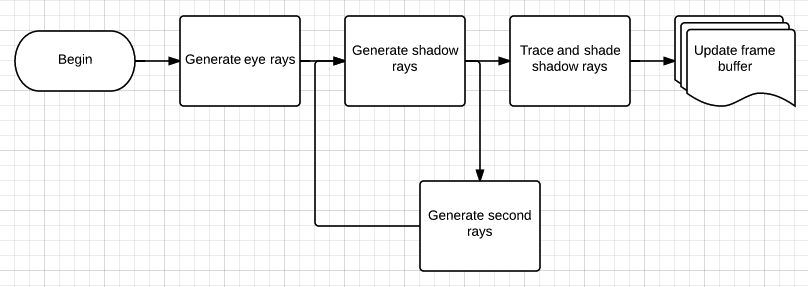
\includegraphics[width=\textwidth] {img1}
$Figure. 1\ Ray\ tracing\ system\ overview$
\end{figure}
\subsubsection{Distribution Policy}
\paragraph{}The distribution of scene is shown in figure $Figure. 2$. We tested the system on CMU’s gates center computer clusters that use AFS file system. Our scene file, a xml description file indicates the distribution policy of geometries in the scene. At this stage, we manually distribute the geometries, but there is the potential of automatic and smart distribution of geometries. We used Open MPI message passing interface for data flow control.
\begin{figure}[h]
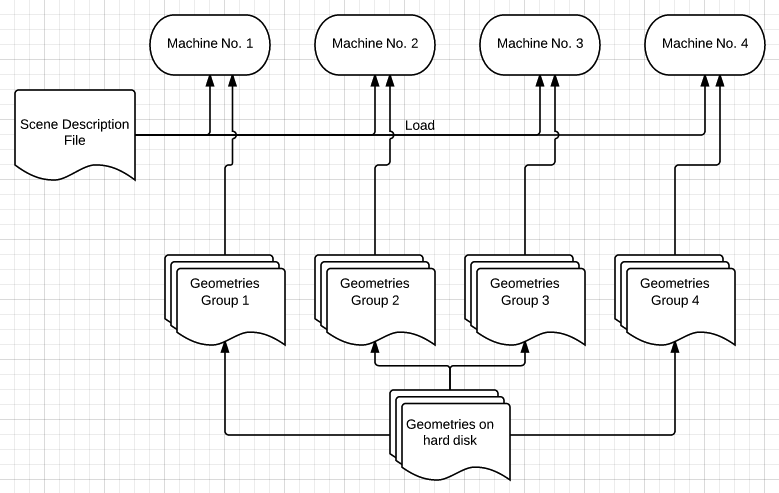
\includegraphics[width=\textwidth] {img2}
$Figure. 2\ System\ distribution\ policy$
\end{figure}

\subsection{Approach 1 - Staged}
\subsubsection{Overview}
\paragraph{}The first approach is a stage by stage algorithm. The idea behind it is to take the advantage of distributed machines across the network. Each of the ray tracing stage is separated. Each of the nodes (machines) in the system performs the exact same operations at the same stage. After each stage, there would be a synchronized blocking communication in between machines for exchanging the required data for next stage. The data would be duplicated across machines. For example, if one eye ray hits multiple root level bounding boxes of different nodes, the eye ray would be duplicated and sent to multiple machines. 
After the stage of tracing and when comes to the stage of shading, each machine / node would update their own local frame buffer, depth buffer and shadow map. Then a gather operations is performed on root node, and framebuffer information from different nodes would be merged.
The system is shown in $Figure 3$.
\begin{figure}[h]
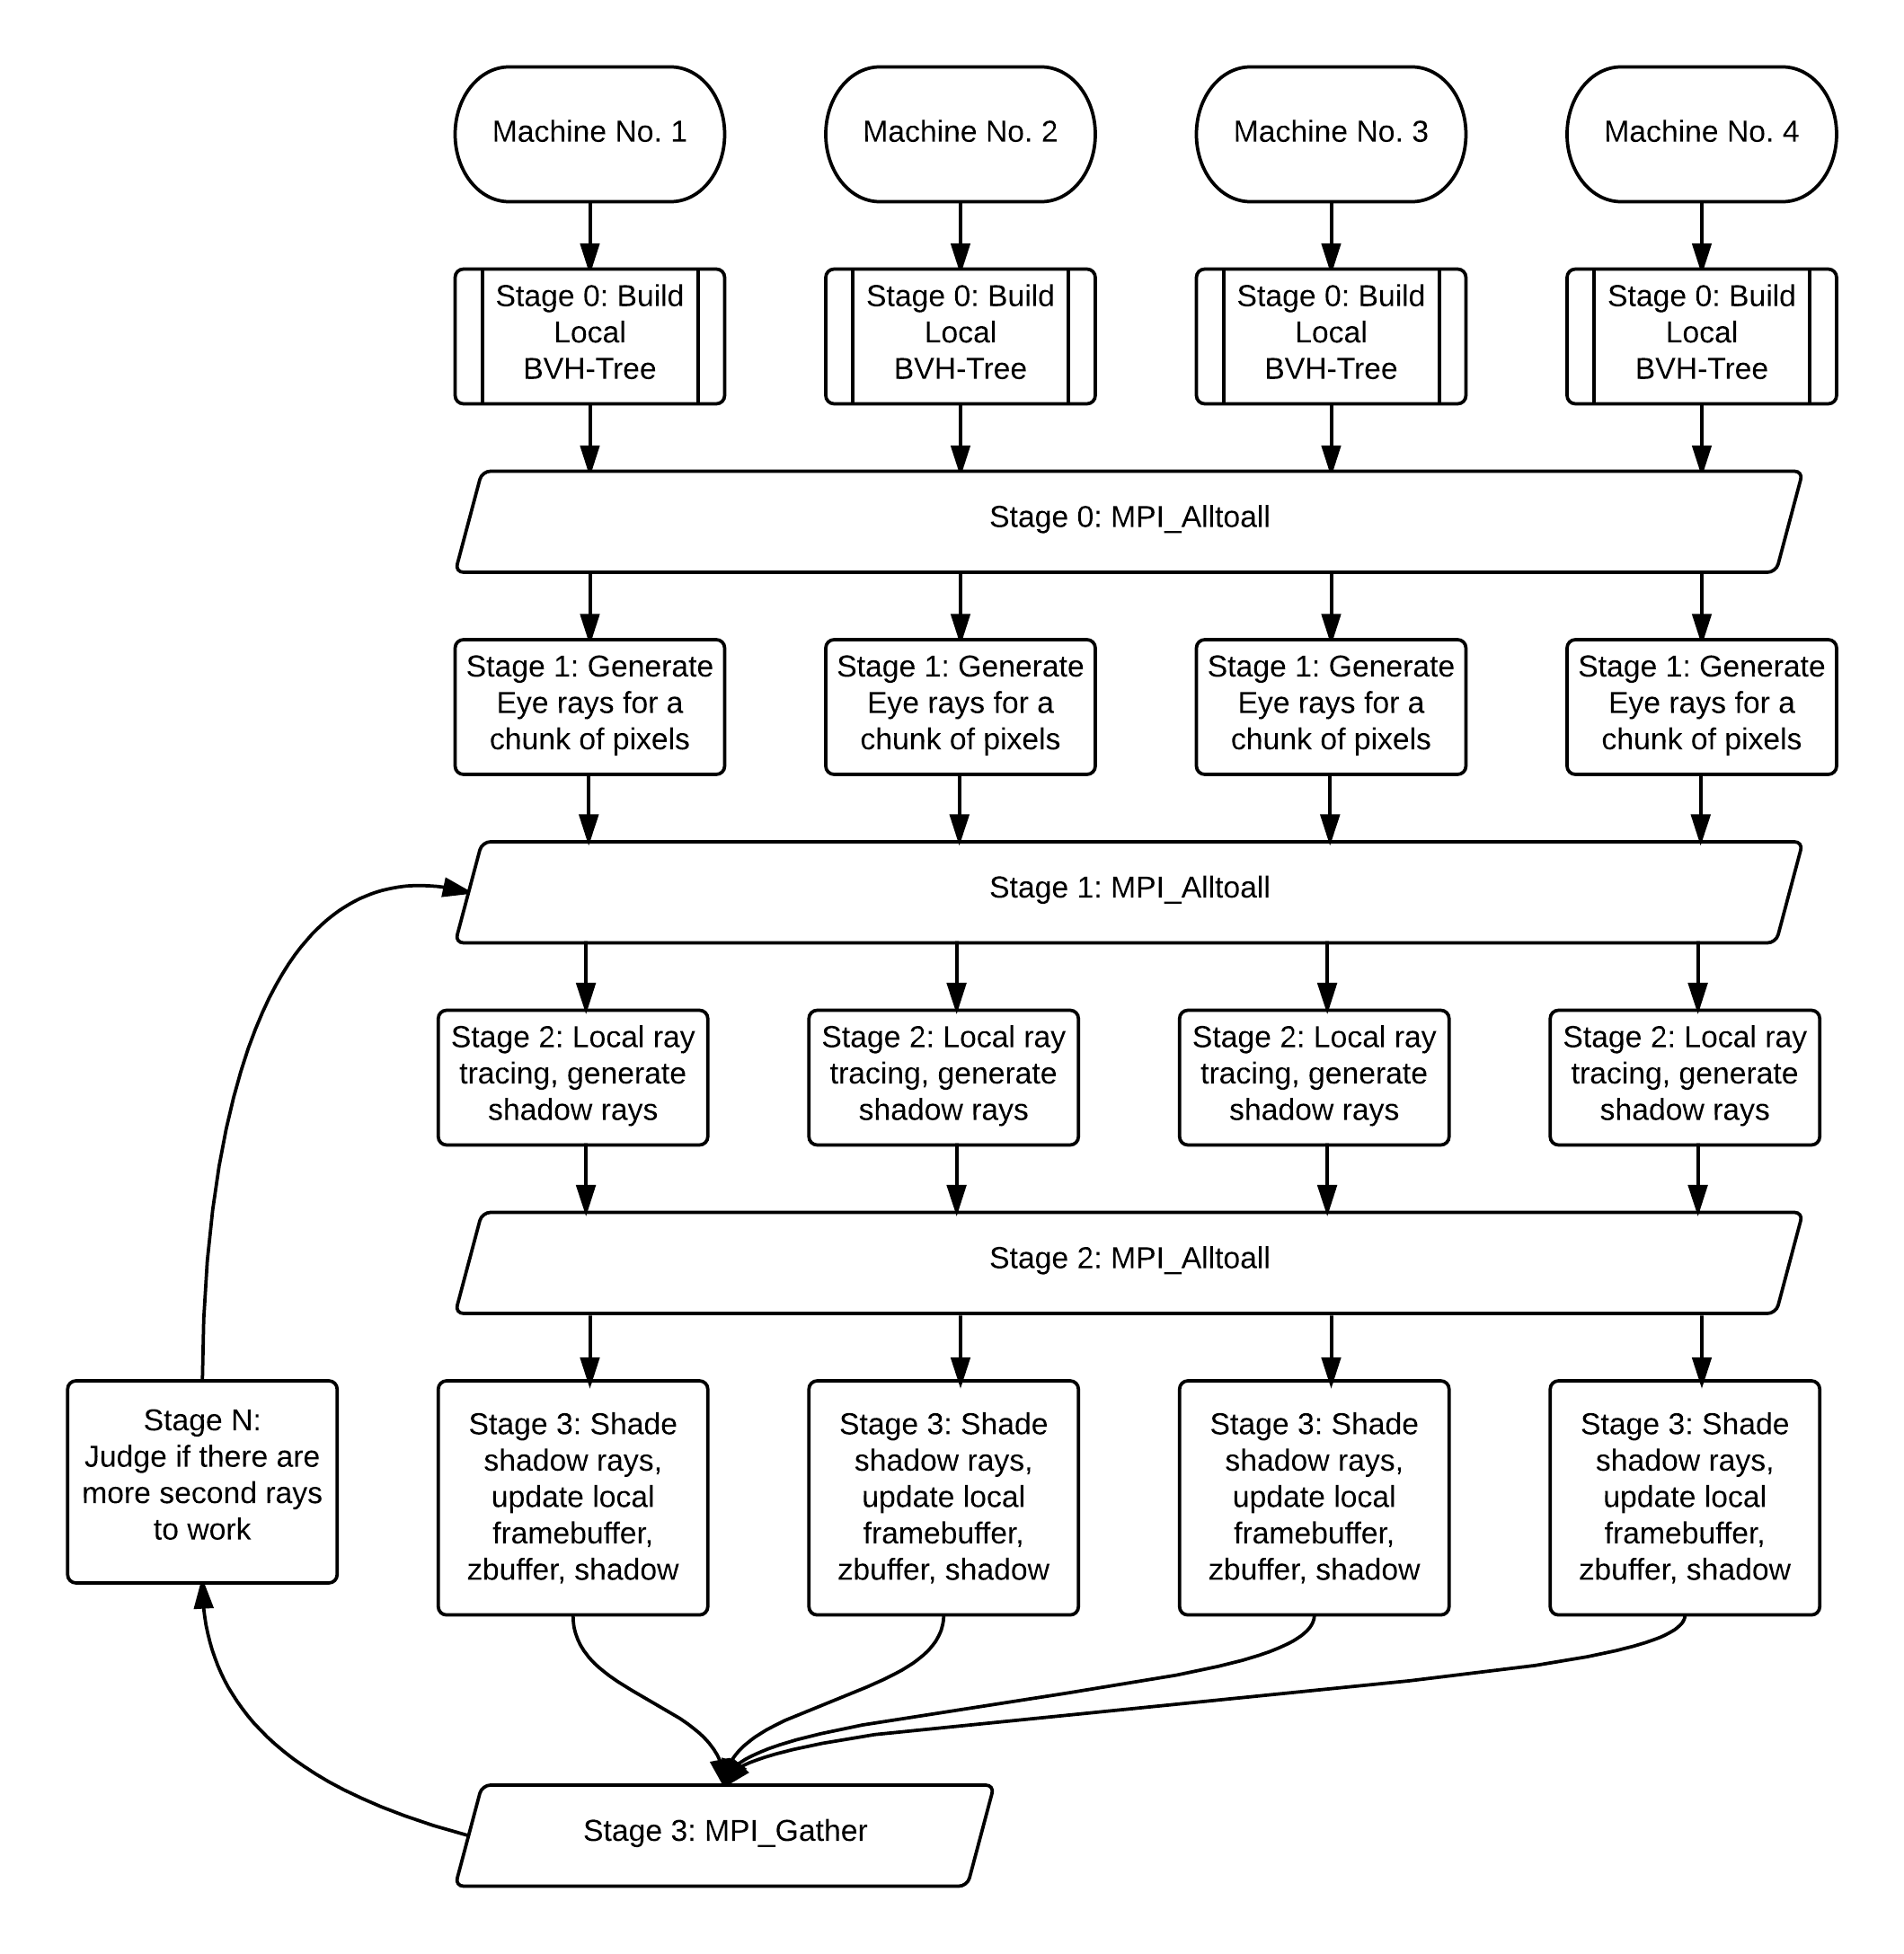
\includegraphics[width=\textwidth]{algo1}
$Figure. 3\ Algorithm 1.\ Workflow\ of\ staged\ system$
\end{figure}
\paragraph{}The assumption behind it is that local ray tracing and shading is fast and cheap and inter-nodes communication is expensive, meanwhile, Open MPI is optimized for large chunk of data exchange. The design assumes that the overhead of increased replicated work is lower than the overhead of increased communication.
\subsubsection{Work Flow}
\paragraph{}The pseudocode is as following, at the end of each function, there would a data exchange with synchronized blocking message passing:
\lstset{language=c++}
\begin{lstlisting}[frame=single]
    void mpiTrace()
    {
        mpiStageDistributeEyeRays();
        mpiAllToAllExchange(eyerays);
        
        mpiStageLocalRayTracing(eyerays);
        mpiAllToAllExchange(shadowrays);
        mpiAllToAllExchange(secondrays);
        
        mpiStageShadowRayTracing(shadowrays);
        mpiGather(framebuffer, root);
       	mpiMergeFrameBuffer();
        
        while (second rays are not done) {
            mpiStageLocalRayTracing(second rays);
            mpiAllToAllExchange(shadowrays);
            mpiAllToAllExchange(secondrays);
            
            mpiStageShadowRayTracing(shadowrays);
            mpiGather(framebuffer, root);
            
            mpiMergeFrameBuffer();
        }
    }
\end{lstlisting}
$Algorithm. 1\ Synchronized\ staged\ based\ path\ tracing$
\subsubsection{Algorithm Discussion}
\paragraph{} The core idea behind the algorithm is to minimize node-to-node communication. Note that the goal is to diminish communication frequency, instead of diminish the communication size. The algorithm would send all rays to all nodes that potentially have an intersection with the rays in the ray list. The sending and receiving of ray data always happen at the same time for all nodes. Once every node gets the ray data needed for ray tracing, it would immediately do local ray tracing, and generate more rays needed for the next stage. 
\paragraph{} Apparently, a major drawback is the duplication of work. Imaging a ray hits the bounding boxes of all nodes, the concept ray would be duplicated and sent to all nodes, each node would do a local tracing and shading, whereas at the final merging stage, there should be only one shading result needed. Therefore for each ray that is sent to $N$ nodes, $N-1$ works are wasted. The ratio of wasted work depends on how many nodes each ray might potentially hit. However, the worst case scenario is all nodes' geometries occupy the whole screen space, and each ray must hits all nodes. This would cause the system to be running as nodes numbers $(N)$ of independent ray tracer, each one has $1/N$ total geometries, plus inter communication overhead. Given the fact that our ray tracer runs reasonably fast on local ray tracing, the performance would not be so bad at first glance.
\paragraph{}However, the second rays could cause further problems since second rays might explode if duplicated works are not reduced. Assuming each first ray hit would generate $m$ more second rays, and each ray would on average hits $n$ geometries, and recursion depth is $k$. For a regular ray tracer, a ray hit would in total cause $m^k$ ray testing, our first algorithm would cause $(n*m)^k$ rays. The increase of workload would be proportional to $n^k$. This would become a disaster if $n$ increases, therefore we expect a relatively bad scalability to this system.
\subsubsection{Future Optimization}
\paragraph{}The problem mentioned in last section however is not completely unsolvable. An optimization might be perform a 

\subsection{Approach 2 - Asynchronous}
\subsubsection{Overview}
\subsubsection{Work Flow}
\subsubsection{Data Communicated}
\subsubsection{Hopping Algorithm}
\paragraph{} One drawbacks of the first approach is the duplicated processing of rays across machine resulting in duplicated works when rays hit multiple bounding boxes. To be specific, in the current design of the system, since model are distributed on each nodes, a ray can potentially hit multiple bounding boxes if the models are close together but on different nodes.  In the first approach, when a ray hits multiple bounding boxes, the ray is sent to multiple node for tracing ans shading independently. This solution not only resulted in extra work in the tracing and shading, it also caused several other issues.
\paragraph{} The first is that the system would need extra state information to decide how to combine the shading results from multiple nodes together into the frame buffer. As mentioned in the above, a depth buffer and a shadow map is required to correctly combine the shading results from multiple machines. 
\paragraph{} The second problem is the duplication of second rays or global illumination rays. For example, when an eye ray hit multiple bounding boxes, it is sent to multiple nodes for processing. Following the ray tracing algorithm, when an eye ray hits a surface, it generates a shadow ray and some number of global illumination rays. In this case, when the eye ray is sent to multiple nodes, each nodes after processing and shading would generate a shadow ray and global illumination rays. However, among all these second rays generated, only one set is actually valid. All the other rays' work would be wasted. In addition, when the depth of global illumination rays gets large, the number of wasted work would grow exponentially. 
\paragraph{} In order to resolve this problem, we devised the following algorithm in processing the rays for the asynchronous system.  Unlike the staged approach, this asynchronous approach allows the rays at each stage to go through multiple iterations since the asynchronous approach is not defined by stages but by iterations.
\paragraph{} The algorithm we devised is quite similar to a single thread ray tracing, but with a tweak, it works on distributed settings as well.  In a single thread ray tracing system, a ray is traced by traversing the BVH tree. Each time during the traversal when a ray hits a surface, a time value $t$ is updated for the ray and the hit surface.  The traversal would continue to other branch of the BVH where the ray also hits the bounding box of the branch, but it can potentially be pruned if the subbranch has $t$ value greater than the existing $t$ value. Our algorithm on the distributed settings mimics this single threaded algorithm.
\paragraph{} First, we devised a strict ordering between nodes using node ID in an increasing order, given node ID is unique across the system. If a ray hits multiple bounding boxes, the ray is always first sent to the node with one of the bounding boxes who has the lowest node ID for processing.  After tracing at the node, the ray would be sent to the node with the next lowest node ID for processing, but with a new time $t$ generated by the tracing on this node. The next node, when tracing the ray, can use this $t$ value to eliminate a large amount of work in tracing. If there is no node bounding boxes with a higher ID that intersects the ray, the ray is considered done and to be sent to master for updating the frame buffer and shadow rays or global illumination rays are generated if needed.  For example, if a ray hits the bounding box of node 0, 2, and 4, the ray would be first sent to node 0, then node 2 and finally node 4. At node 4, it sees that no other node with bounding boxes that intersect with this ray and a higher node ID, it considers the ray to be done.
\paragraph{} In this way, the system remains stateless and only generates rays that are needed.

\subsubsection{Future Optimization}
\section{Result}

%%%%%%%%%% BIBLIOGRAPHY %%%%%%%%%%


\bibliographystyle{plain}
\bibliography{references}
\addcontentsline{toc}{section}{References}

\end{document}